The development of TeamJob represents a significant undertaking in modern web application development, but the project's true value lies not merely in its technical implementation, but in the insights it provides about software engineering practices, architectural decision-making, and the challenges of creating organizational tools.
This discussion critically examines the project's successes, limitations, and broader implications.


\section{Architectural Decisions and Their Implications}\label{sec:architectural-decisions-and-their-implications}

Spring Boot selected (Section~\ref{sec:technology-choices}); MVC structure clarified, service layer introduced (Section~\ref{sec:testing-strategy}); JWT authentication implemented (Section~\ref{sec:security-implementation}); calendar system designed for RFC 5545 (Section~\ref{sec:calendar-functionality}); PostgreSQL and H2 configured (Section~\ref{sec:database-design2}); Thymeleaf-based UI chosen (Section~\ref{sec:user-experience-/-user-design}); comprehensive testing applied (Section~\ref{sec:testing-strategy}); technology stack evaluated (Section~\ref{sec:technology-choices}).


\section{Security Implementation}\label{sec:security-implementation}

The implementation of JWT-based authentication represents a modern, state-less approach to authentication.
This was further intensified by the reluctance to manually manage sessions or establish a dedicated system for this purpose.
The issue of improper configuration of the filter chain has frequently emerged; however, with the current setup, such complications should no longer arise during application usage.

Another potential issue is the implementation of distinct account storage and logging systems.
This approach may not be compatible with organizations that employ a single account per individual across all their systems.
This challenge could be addressed by extensively modifying the source code, given that the program is entirely open to modification and redistribution.


\section{Calendar Functionality}\label{sec:calendar-functionality}

The calendar system represents the project's most complex component, and its implementation reveals both the power and limitations of the chosen approach.
The RFC 5545 compliance for recurring events, while technically correct in the backend implementation, introduced significant complexity that affected the frontend display development.
The availability calculation algorithms, while efficient for moderate datasets, may not scale to enterprise-level deployments with thousands of users and events.

The powerful filtering system offers users the ability to identify the most suitable schedule.
However, the challenge lies in the extensive filtering required.
An idea emerged later in the project to establish predefined tag groups tailored for specific student demographics, such as first-year students in the XYZ program.
Students would have the opportunity to adjust these tags to meet their specific requirements.
The implementation of this feature has been canceled due to time constraints.


\section{Database Design}\label{sec:database-design2}

Employing a PostgreSQL database within a Docker container was a strategically beneficial decision; however, it introduced a certain level of complexity when working within a local environment utilizing an H2 database.
Considerable time was devoted to the issues of \texttt{ application.properties} and \texttt{ application-test.properties}.
Eventually, the configuration was adapted to utilize the \texttt{.env} file for the deployed environment, while locally-selected variables were employed for test cases.

The current method for implementing the \texttt{ user\_roles} table and ``tags'' tables is functional.
However, it may ultimately complicate the comprehension of the entire system and its operational mechanics.

\newpage

\section{User Experience / User Design}\label{sec:user-experience-/-user-design}

The user interface design prioritizes functionality over aesthetics, which is appropriate for an organizational tool, but may limit adoption in environments where user experience is of the utmost importance.
The use of a Thymeleaf-based methodology ensures robust performance and security; however, it restricts the level of dynamic interactivity anticipated by modern users.
This limitation could be addressed by transitioning to the currently prevalent JavaScript frameworks.
However, the author lacked the requisite expertise in such frameworks, and temporal constraints precluded this transition.

\begin{figure}[htbp]
    \centering
    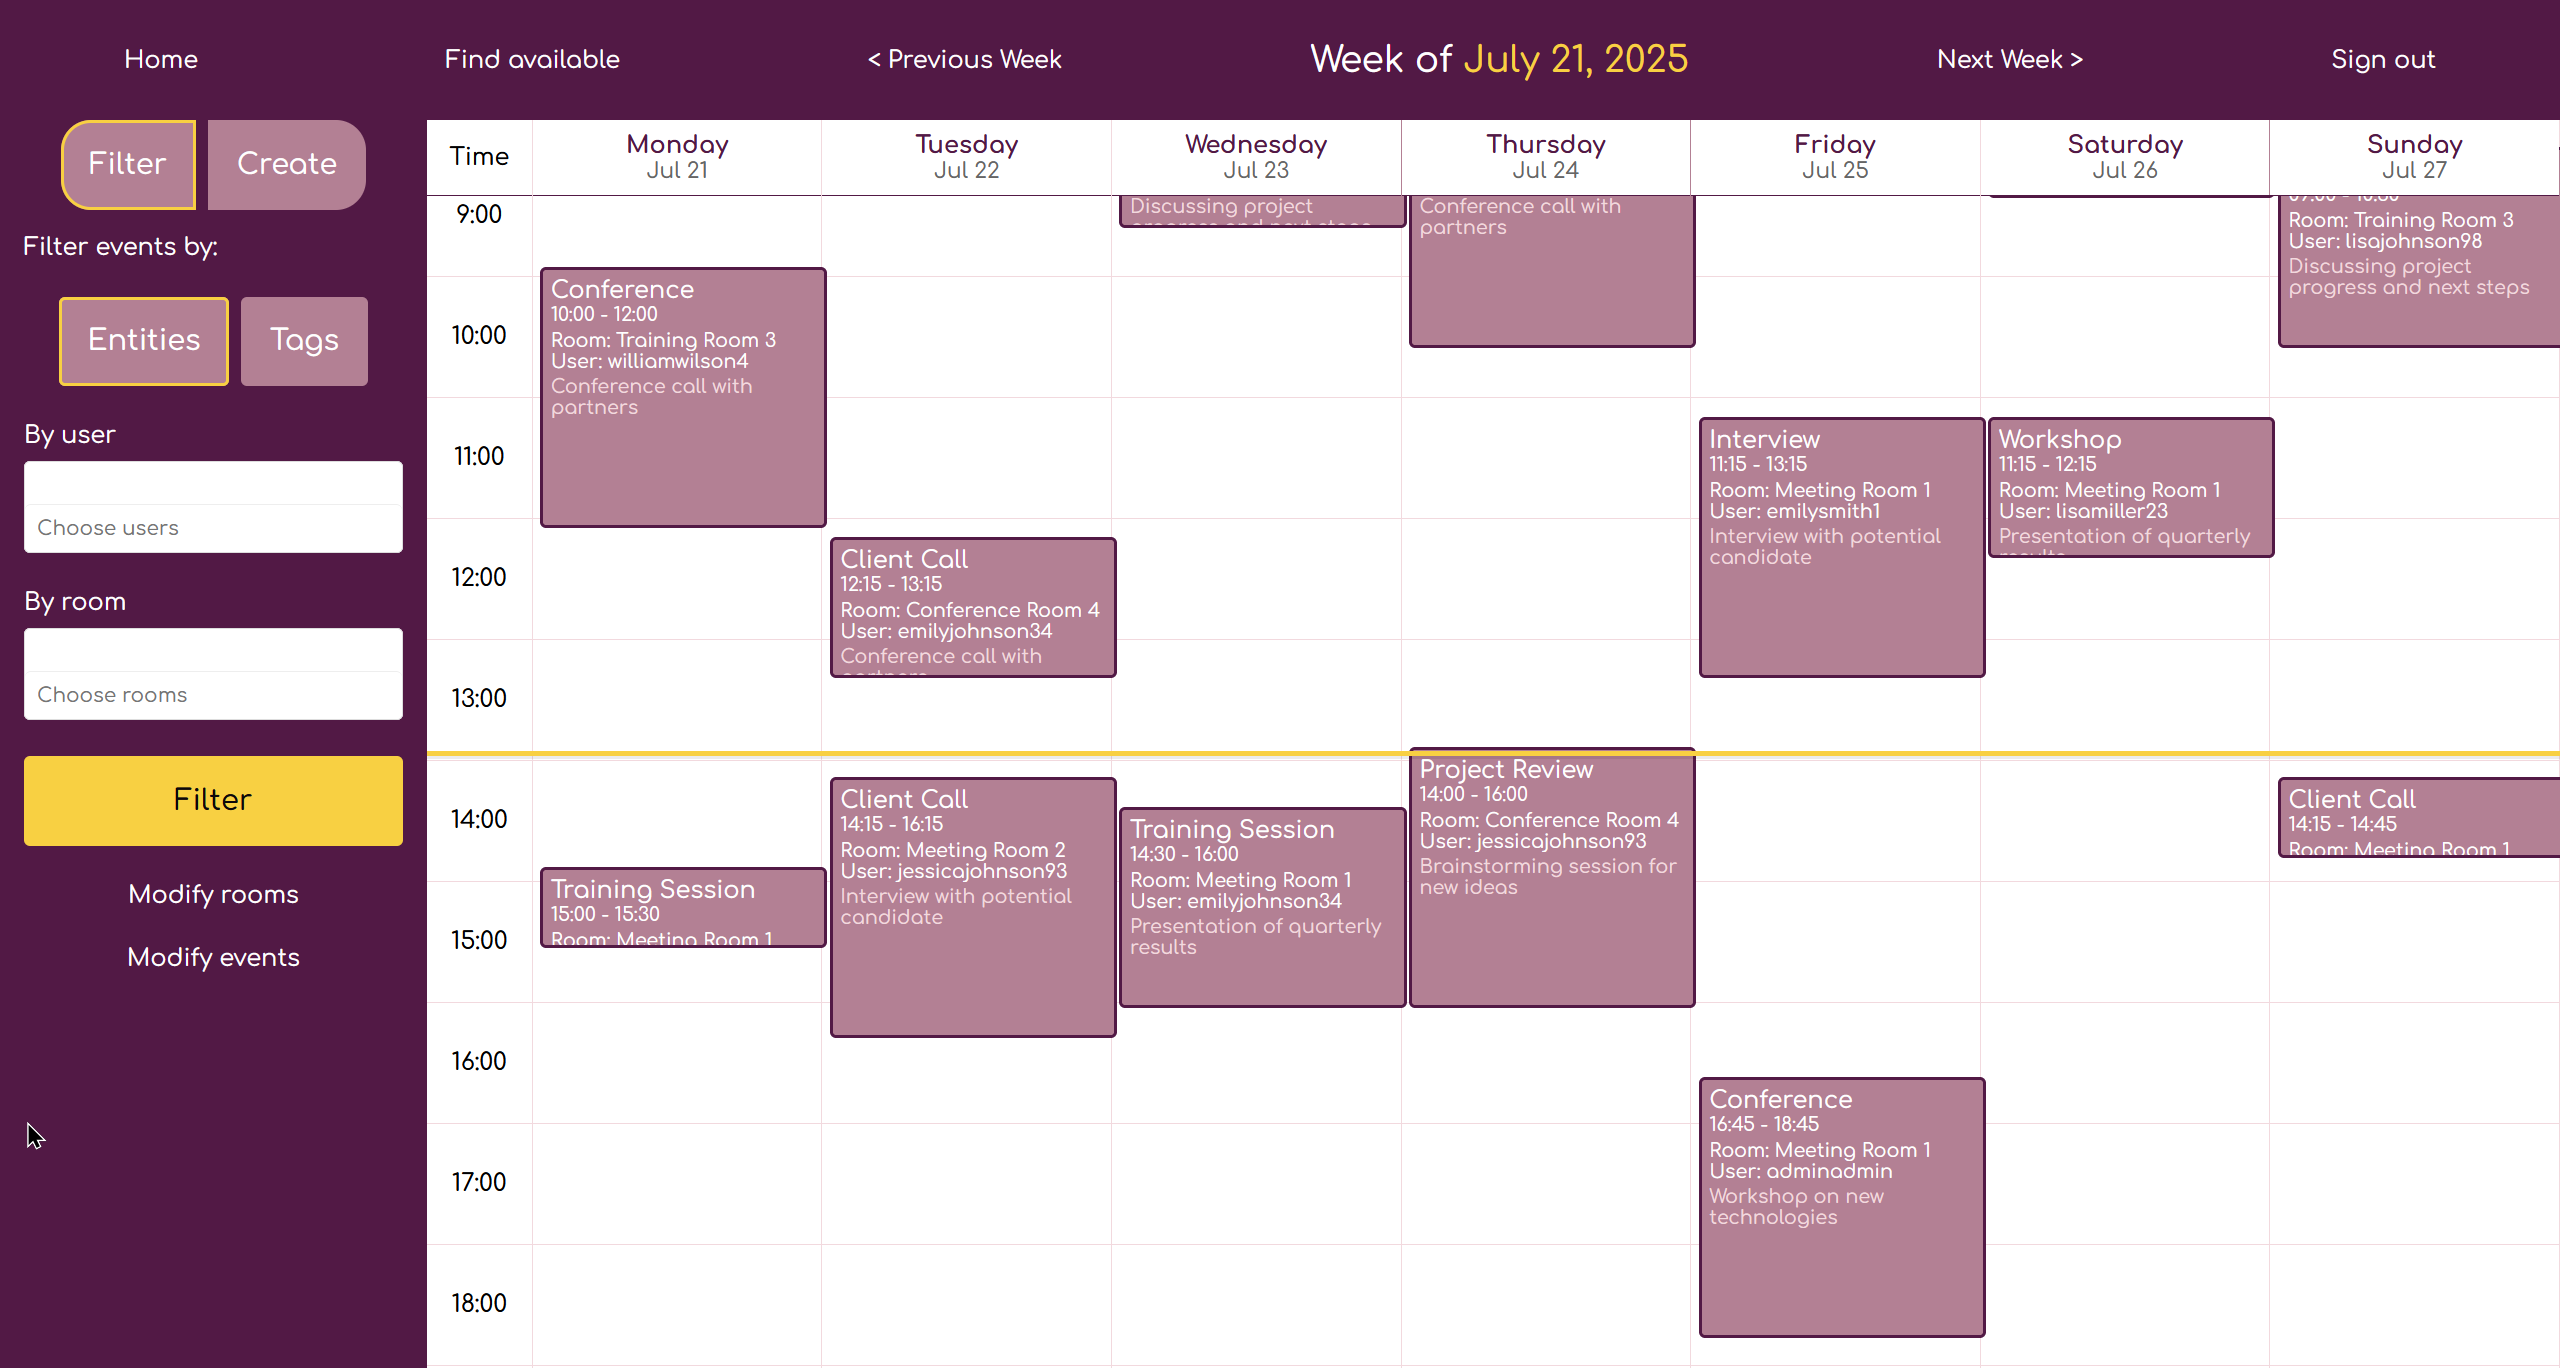
\includegraphics[width=0.8\textwidth]{Week_view}
    \caption{Weekly calendar view interface of the TeamJob application displaying scheduled events in a grid format.}
    \label{fig:week-view}
\end{figure}

The creation of an effective calendar interface presents the challenge of displaying scheduling data in a way that is both clear and user-friendly.
Feedback from an expert within the design domain has been positively received regarding the UI elements~\ref{fig:week-view} of the application, particularly applauding the selection of color schemes and the intuitive nature of the navigation system.


\section{Testing Strategy}\label{sec:testing-strategy}
The testing methodology employed within TeamJob was characterized by a comprehensive and detailed examination that included the service, controller, and repository layers.

\textbf{Test Data Management:} Each test class independently configures and dismantles its data to ensure both isolation and repeatability.
Helper methods are used to create realistic test entities, and the database is meticulously cleaned before and after each test to prevent cross-test contamination.

\textbf{Service Layer Testing:} The \texttt{CalendarServiceImplTest} class employs JUnit 5 and Mockito to thoroughly evaluate the business logic inherent in the calendar service.
The service logic is effectively isolated through the injection of mock repositories, and comprehensive test data is generated for users, rooms, and events.
The testing protocol covers various scenarios, such as event conversion, recurrence rules, filtering, and overlapping events, to verify that the core scheduling logic functions correctly.

\textbf{Controller Layer Testing:} The \texttt{RestConfigControllerTest} class employs Spring Boot's \texttt{@SpringBootTest} and \texttt{@AutoConfigureMockMvc} to execute integration testing on REST endpoints.
These assessments simulate authentic HTTP requests through the utilization of MockMvc, validating authentication, authorization, and accurate handling of event creation, including the backend processing of recurring events.
JWT tokens are systematically generated for a variety of user roles to evaluate access control mechanisms.
The validation procedures ensure that actions are executable exclusively by users with the necessary roles and that the API delivers precise responses to both legitimate and illegitimate requests.

\textbf{Repository Layer Testing:} The \texttt{EventRepositoryTest} and \texttt{RoomRepositoryTest} classes utilize \texttt{@DataJpaTest} to assess the persistence layer through an in-memory database.
Validates custom query methods designed to locate events based on time, room, title, and tags, as well as to detect overlapping events.
These tests verify the precision of the repository logic and the ability of the database schema to facilitate the necessary queries.

\begin{table}[htbp]
    \centering
    \caption{Test Suite Results Summary}
    \begin{tabular}{|p{0.5\textwidth}|c|}
        \hline
        \textbf{Test Category}    & \textbf{Pass Rate}     \\
        \hline
        Application Context Tests & 100\% (1/1)            \\
        \hline
        Controller Tests          & 100\% (9/9)            \\
        \hline
        Repository Tests          & 100\% (12/12)          \\
        \hline
        Service Tests             & 100\% (25/25)          \\
        \hline
        \textbf{Total}            & \textbf{100\% (47/47)} \\
        \hline
    \end{tabular}
    \label{tab:test-results}
\end{table}


\section{Technology Choices}\label{sec:technology-choices}

The technology stack represents a solid choice for the project requirements, but each component introduces both benefits and trade-offs.
Spring Boot eases developer productivity and offers a wide array of extensions along with support for various features.
Despite its extensive customization capabilities, alternative back-end frameworks may present configuration options that are more straightforward.
PostgreSQL is the highly popular database for modern applications.
It is often used for both small-scale applications and enterprise applications.\cite{ThebenefitsofPostgreSQL,GerritMeyer2025}

The use of Thymeleaf as a templating engine guarantees substantial security and performance.
However, it limits the dynamic user experience that is often required by modern applications.
In contrast, contemporary JavaScript frameworks enable the development of more dynamic pages, facilitating easier reuse of design patterns and additional features.
